% FUNDAMENTAÇÃO: apresente os conceitos e as pesquisas relacionados ao tema.
\section{Fundamentação Teórica}
\label{sec:fundamentacao}

Defina os conceitos necessários à compreensão da pesquisa. Organize a revisão
por assuntos, compare as contribuições dos autores e identifique a lacuna que
seu trabalho pretende investigar. Cite as fontes efetivamente consultadas.

\subsection{Citações e referências}

% \citeonline insere o nome do autor na frase; \cite usa parênteses.
Exemplo do comando de citação no corpo da frase:
\citeonline{SilvaNeto2019Credibility}. Exemplo entre parênteses:
\cite{SilvaNeto2019Credibility}. Os dados são recuperados automaticamente
do arquivo de bibliografia.

\subsubsection{Citação em bloco}

O ambiente a seguir demonstra a formatação de uma citação longa. O conteúdo
é uma instrução de preenchimento, não uma transcrição de uma obra publicada.

\begin{citacao}
  Substitua este parágrafo pelo trecho exato da obra consultada. Identifique
  a autoria e a localização do trecho na fonte. Não mantenha este texto de
  orientação como se fosse uma citação real. Confira a transcrição e os
  requisitos de apresentação adotados pelo seu curso antes da entrega.
\end{citacao}

% Para indicar uma página real, use \cite[p.~número]{chave-da-obra}.
Não digite a lista de referências manualmente: ela é produzida a partir das
citações presentes no documento. As referências antigas mantidas no banco
de exemplos não representam uma verificação das normas em vigor.

% EXEMPLO -- as duas figuras abaixo vieram do modelo original e não têm
% relação com o seu tema. Troque as imagens, as legendas e as fontes.
\subsection{Exemplos de gráficos}

As Figuras~\ref{graf1} e~\ref{graf2} demonstram a inclusão de imagens.
Troque os arquivos, os títulos e as fontes pelos materiais da sua pesquisa.
A numeração é automática; não escreva o número dentro da legenda.

\begin{figure}[htb]
  \centering
  \caption{Atendimento na educação básica por dependência administrativa
  no município de Avaré, 2014}
  \label{graf1}
  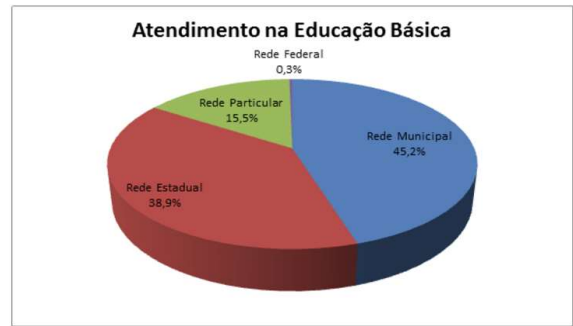
\includegraphics[width=0.85\linewidth]{imagens/grafs_1.png}
  \fonte{Secretaria Municipal de Educação de Avaré (2014), conforme o exemplo original.}
\end{figure}

\begin{figure}[htb]
  \centering
  \caption{Distribuição do número de matrículas por etapas da educação básica
  no município de Avaré, 2014}
  \label{graf2}
  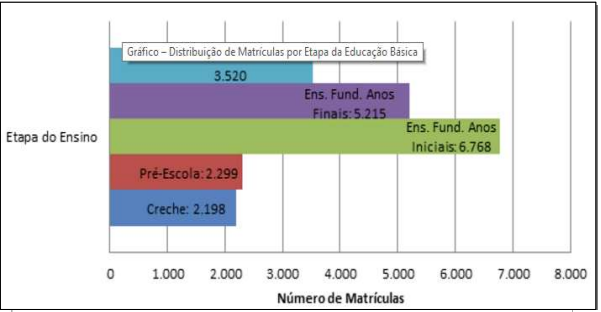
\includegraphics[width=0.85\linewidth]{imagens/grafs_2.png}
  \fonte{Secretaria Municipal de Educação de Avaré (2014), conforme o exemplo original.}
\end{figure}

% EXEMPLO -- figura de demonstração; confira a procedência antes de reusar.
\subsection{Exemplo de ilustração}

A \autoref{fig_arranjo} demonstra uma imagem acompanhada de uma citação na
indicação de fonte. Discuta no texto o que cada figura acrescenta à pesquisa,
em vez de apenas inseri-la.

\begin{figure}[htb]
  \centering
  \caption{Arranjo produtivo local da banana orgânica}
  \label{fig_arranjo}
  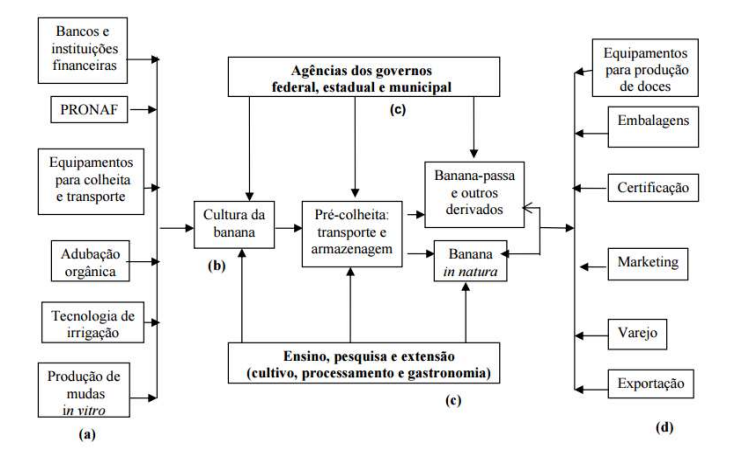
\includegraphics[width=0.8\linewidth]{imagens/fig_exemplo.png}
  \fonte{\citeonline{limaarranjo}.}
\end{figure}
